\begin{frame}[t]{Database for Inversion}
Deep Learning methods are fast, but they \textbf{require a massive training dataset}.
\vspace{0.2cm}

We need to solve Maxwell's equations. \textcolor{red}{3D simulations are expensive}. Reduce dimensionality using Fourier or Hankel transforms. (So called 1.5D and 2.5D formulations).
\vspace{0.2cm}

\visible<2-3>{Methods to solve PDEs: FEM and IGA.
\begin{itemize}
\item IGA provides smoother solutions.
\item \textcolor{red}{IGA increases cost of LU factorization}
\end{itemize}
\vspace{0.2cm}

\textbf{rIGA} decreases the cost of LU factorization.
\vspace{0.2cm}

\begin{thebibliography}{1}
\bibitem{Dani} D. Garcia et al. The value of continuity: Refined isogeometric analysis and fast direct solvers. Computer Methods in Applied Mechanics and Engineering, 316: 586–605, 2017.
\end{thebibliography}
}
\vspace{0.2cm}

\visible<3>{In this Section, \textbf{we use rIGA methods to generate a database for DL inversion.}}
\end{frame}


\begin{frame}[t]{rIGA Database Generation}
\begin{columns}
    \begin{column}{0.35\textwidth}
    \begin{figure}[!h]
	\centering
	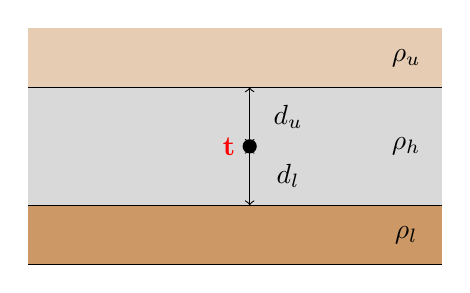
\begin{tikzpicture}[scale=1.5]
\draw (0,0) rectangle (3.5,2);

\fill[white!20!brown] (0,0) rectangle (3.5,0.5);
\fill[white!70!gray] (0,0.5) rectangle (3.5,1.5);
\fill[white!60!brown] (0,1.5) rectangle (3.5,2);


%\draw[red, line width=0.5 mm] (0.75,1.5) .. controls (1.15,1.1) .. (1.85,1) node (n1) at (0.85,1.6) {$\mathbf{t}$};
\draw[black, line width=0.1 mm] (0,0.5) -- (3.5,0.5);
\draw[black, line width=0.1 mm] (0,1.5) -- (3.5,1.5);

\fill[black] (1.875,1) circle (0.06cm);
\node (d_u) at (1.7,1) {\textcolor{red}{$\textbf{t}$}};
\draw[<->] (1.875,1.02) -- (1.875,1.5);
\node (d_u) at (2.2,1.25) {$d_u$}; 
\draw[<->] (1.875,0.98) -- (1.875,.5);
\node (d_u) at (2.2,0.75) {$d_l$};
\node (rho) at (3.2,1.75) {$\rho_u$};
\node (rho) at (3.2,0.25) {$\rho_l$};
\node (rho) at (3.2,1) {$\rho_h$};
\end{tikzpicture}

	\label{fig:param}
	\end{figure}
    \end{column}
    \begin{column}{0.5\textwidth}
        {\footnotesize $\rho_u \in [1,10^2] \Omega \cdot m$: Upper layer resistivity}\\
        \vspace{0.3cm}
        {\footnotesize $\rho_h \in [1,10^2] \Omega \cdot m$: Central layer resistivity}\\
        \vspace{0.3cm}
        {\footnotesize $\rho_l \in [1,10^2] \Omega \cdot m$: Lower layer resistivity}\\
        \vspace{0.3cm}
        {\footnotesize $d_u \in [10^{-2},10] m$: Vertical distance to upper layer}\\
        \vspace{0.3cm}
        {\footnotesize $d_l \in [10^{-2},10] m$: Vertical distance to lower layer}
    \end{column}
\end{columns}
\vspace{0.2cm}

\begin{itemize}
\item Generate $100.000$ samples and compute their measurements.
\vspace{0.2cm}
\item We need $\simeq 56$h to generate the database.
\end{itemize}

\begin{thebibliography}{2}
\bibitem{Ali} A. Hashemian, D. Garcia, J. A. Rivera and D. Pardo. Massive database generation for 2.5 D borehole electromagnetic measurements using refined isogeometric analysis. Computers \& Geosciences 155, 104808, 2021.
\end{thebibliography}
\end{frame}


%\begin{frame}{PREGUNTAS y COMENTARIOS}
%No se nada de IGA. Por eso no me atrevo a poner nada mas. Y si me preguntan algo de esto quiero saber como contestar. Vamos, quiero saber que frase decir para quedar bien.
%\vspace{0.5cm}
%
%La verdad que no se como poner los resultados. O mejor dicho, que mas poner.
%\vspace{0.5cm}
%
%Tengo varias preguntas para hacerte sobre este topic. Quiero intentar al menos llevar un par de conceptos preparados.
%\end{frame}




%\begin{frame}{Isogeometric Analysis}

%Una slide donde explique que es rIGA de una manera muy facil (tengo que entenderlo yo) y sus ventajas
%
%Que es lo que yo he contribuido en este trabajo? En la parte de resolver el problema inverso? A mi me daban unos datos y yo les daba otros. Creo que em daban att/ph y les daba las resistividades????? Lo que hacia era ejecutar una tabla
%
%Poner directamente los resultados obtenidos. Pondria los dos graficos de la generacion de la base de datos y ya. Tal vez tiempos y asi.
%
%POR QUE HAY UNA CORRELACION LINEAL ENTRE ATENUATION Y PHASE????????

%\end{frame}

